\documentclass[UTF8,a4paper,11pt]{ctexart}

\usepackage[margin=2.1cm]{geometry}
\usepackage{amsmath}
\usepackage{amssymb}
\usepackage{array}
\usepackage{booktabs}
\usepackage{longtable}
\usepackage{xcolor}
\usepackage{hyperref}
\usepackage{listings}
\usepackage{tikz}
\usepackage{tikz-timing}
\usetikzlibrary{positioning,arrows.meta,calc,shapes.geometric,fit,backgrounds}

\hypersetup{
  colorlinks=true,
  linkcolor=blue!60!black,
  urlcolor=blue!60!black
}

\definecolor{codebg}{HTML}{F3F3F3}
\definecolor{accent}{HTML}{C0392B}
\definecolor{regwrite}{HTML}{E67E22}
\definecolor{regread}{HTML}{2980B9}
\definecolor{regsecret}{HTML}{8E44AD}

\lstset{
  basicstyle=\ttfamily\footnotesize,
  backgroundcolor=\color{codebg},
  frame=single,
  framesep=4pt,
  framerule=0pt,
  showstringspaces=false,
  breaklines=true,
}

\newcommand{\hex}[1]{\texttt{0x#1}}
\newcommand{\reg}[1]{\texttt{#1}}

\title{APP\_I2CEEPROM 设计文档\\
       \large TX32F01 仿真加密 I\textsuperscript{2}C EEPROM 固件}
\author{Codex 生成}
\date{\today}

\begin{document}
\maketitle
\tableofcontents
\newpage

\section{项目目标}

\subsection{一句话总览}

把一颗 TX32F01（Cortex-M0、24 MHz、32 KB Flash、4 KB SRAM）做成一个
\textbf{16 KB I\textsuperscript{2}C EEPROM 仿真器}，从总线视角看与
24LC128 兼容，并在内部增加两个真实 EEPROM 不具备的杀手特性：

\begin{enumerate}
    \item \textbf{透明 AES-128-CTR 加密区}：地址 \hex{3F00}--\hex{3FFB}（252 字节）
          写入 Flash 前自动加密；读出时自动解密给主控。
          \textbf{把芯片焊下来用编程器读 Flash，看到的是密文。}
    \item \textbf{单调递增计数器}：地址 \hex{3FFC}--\hex{3FFF}（4 字节，big-endian）。
          读：返回当前计数值；写：忽略数据，计数器 $+1$。用于固件防回滚、
          反重放攻击、序号管理。
\end{enumerate}

\subsection{为什么是这个芯片}

这颗 MCU 的算力和资源（24 MHz、32 KB / 4 KB）与 1980 年代末期高端 EEPROM
控制器接近。把这种"小芯片做储存控制器"的活做出来，比再写一个 PWM 闪灯
demo 工程含金量高得多——而且复制思路就能做出 SPI NOR / 1-Wire EEPROM /
智能卡等一整族"仿真型"产品。

\subsection{三层架构}

\begin{center}
\begin{tikzpicture}[
    layer/.style={rectangle,draw,thick,minimum width=12cm,minimum height=1.3cm,
                  rounded corners=2pt,align=center},
    arrow/.style={-{Stealth[length=3mm]},thick}
]
\node[layer,fill=blue!8]   (app) at (0,3)    {APP / 协议层 \\ \footnotesize EEPROM 协议状态机、加密策略、计数器语义};
\node[layer,fill=green!8]  (bsp) at (0,1.4)  {BSP / 板级支持 \\ \footnotesize I\textsuperscript{2}C 从机硬件初始化 + ISR、UART、引脚映射};
\node[layer,fill=orange!8] (hal) at (0,-0.2) {HAL / 厂家驱动 \\ \footnotesize SCU / GPIO / I\textsuperscript{2}C / UART / Flash 寄存器封装};
\node[layer,fill=gray!12]  (hw)  at (0,-1.8) {Hardware \\ \footnotesize 寄存器：\hex{40001000} SCU / \hex{49005000} I\textsuperscript{2}C / \hex{49002000} UART / \hex{40008000} Flash};

\draw[arrow] (app) -- (bsp);
\draw[arrow] (bsp) -- (hal);
\draw[arrow] (hal) -- (hw);
\end{tikzpicture}
\end{center}

这套分层和 \texttt{APP\_SPINOR} 完全一致，是上次项目验证过的范式。

\section{硬件接线}

\subsection{引脚分配（避开 SWD 引脚）}

\begin{center}
\begin{tabular}{lll}
\toprule
\textbf{信号} & \textbf{TX32F01 引脚} & \textbf{说明} \\
\midrule
I\textsuperscript{2}C SCL & GPIO1.PIN05 & 同步时钟，主机驱动 \\
I\textsuperscript{2}C SDA & GPIO1.PIN06 & 双向数据线 \\
UART TX  & GPIO3.PIN07 & 调试日志，115200 8N1 \\
UART RX  & GPIO3.PIN06 & 未用 \\
LED      & GPIO0.PIN03 & 500\,ms 翻转，心跳指示 \\
SWDIO    & GPIO0.PIN00 & \textbf{保留，不可挪用} \\
SWCLK    & GPIO0.PIN01 & \textbf{保留，不可挪用} \\
\bottomrule
\end{tabular}
\end{center}

I\textsuperscript{2}C 引脚选择依据：vendor 的 \texttt{9.IIC/5.Slave\_IAP} demo
就用这两个引脚作为 I\textsuperscript{2}C 从机配置，已经验证过 AF 路径
可用。

\subsection{典型外部接线图}

\begin{center}
\begin{tikzpicture}[
    chip/.style={rectangle,draw,thick,minimum width=3.5cm,minimum height=4.5cm,align=center},
    host/.style={rectangle,draw,thick,minimum width=2.8cm,minimum height=2.6cm,
                 fill=blue!5,align=center},
    pin/.style={font=\footnotesize}
]
\node[chip,fill=orange!10] (mcu) at (0,0) {};
\node[anchor=north] at (mcu.north) {\textbf{TX32F01}};
\node[anchor=south] at (mcu.south) {\footnotesize 自定义 EEPROM};

\node[host] (h) at (6,0) {};
\node[anchor=north] at (h.north) {\textbf{Host}};
\node[anchor=south] at (h.south) {\footnotesize MCU / FPGA / PC};

\draw[thick] (mcu.east|-0,1.5)   -- node[pin,above]{SDA} (h.west|-0,1.5);
\draw[thick] (mcu.east|-0,0.6)   -- node[pin,above]{SCL} (h.west|-0,0.6);
\draw[thick] (mcu.east|-0,-0.4)  -- node[pin,above]{GND} (h.west|-0,-0.4);

\node[pin,anchor=east] at (mcu.east|-0,1.5) {PIN06};
\node[pin,anchor=east] at (mcu.east|-0,0.6) {PIN05};

\node[draw,circle,inner sep=0,minimum size=4mm,fill=yellow] at (-1.2,-1.2) {};
\node[pin,anchor=east] at (-1.2,-1.2) {LED \footnotesize GPIO0.03 \quad};

\draw[->,thick,gray!60] (-1.4,1.8) -- (-2,2.4) node[pin,above,black]{UART debug 115200};
\end{tikzpicture}
\end{center}

SCL/SDA 任意一端各需 4.7\,k$\Omega$ 上拉到 3.3\,V。多数 PC 端 USB-I\textsuperscript{2}C
桥（CH341、Bus Pirate、FT2232）的板载已经做了上拉，不需额外。

\section{地址空间与特殊区}

\subsection{Flash 物理布局}

TX32F01 总共 32 KB Flash，划分如下：

\begin{center}
\begin{tabular}{lll}
\toprule
\textbf{物理地址} & \textbf{大小} & \textbf{用途} \\
\midrule
\hex{01000000}--\hex{010017FF} & 6\,KB  & 固件代码 + RO 数据 \\
\hex{01001800}--\hex{010057FF} & 16\,KB & \textbf{host 可见 EEPROM} \\
\hex{01005800}--\hex{01007FFF} & 10\,KB & 保留 \\
\bottomrule
\end{tabular}
\end{center}

\subsection{Host 可见的逻辑布局}

主控看到的 16 KB 地址空间内部分三种区域，但**不需要知道哪是哪**——
读写语义和普通 EEPROM 一致。

\begin{center}
\begin{tikzpicture}[
    region/.style={rectangle,draw,thick,minimum width=11cm,minimum height=1cm,
                   font=\small},
    note/.style={font=\footnotesize\itshape}
]
\node[region,fill=green!10]  (plain) at (0,3)    {普通区 \hex{0000}--\hex{3EFF}（15\,872 字节，明文存储）};
\node[region,fill=purple!10] (enc)   at (0,1.8)  {加密区 \hex{3F00}--\hex{3FFB}（252 字节，AES-128-CTR）};
\node[region,fill=red!10]    (ctr)   at (0,0.6)  {计数器 \hex{3FFC}--\hex{3FFF}（4 字节 BE，写则 +1）};

\node[note] at (0,4.2) {读：返回 Flash 原值\quad 写：直接编程 Flash};
\node[note] at (0,0.0) {读：返回最新计数值\quad 写：忽略数据，计数器自动 +1};
\end{tikzpicture}
\end{center}

\subsection{加密区设计细节}

\textbf{密钥派生}：固件启动时从 Flash NVR 寄存器读出 \hex{DIEID0}\dots\hex{DIEID3}
（共 128 bit），与一个固件版本字面量混合，三轮 XOR + 循环左移生成 16 字节
AES 主密钥。

\[
  \mathrm{key}[16] = \mathrm{Mix}\left(
    \mathrm{DIEID0}\,\|\,\mathrm{DIEID1}\,\|\,\mathrm{DIEID2}\,\|\,\mathrm{DIEID3}\,;
    \;\text{"TX32F01:I2CEE:01"}
  \right)
\]

特性：
\begin{itemize}
    \item \textbf{密钥永不离开芯片}：固件代码不存储密钥，每次启动重新派生。
    \item \textbf{设备唯一}：不同 chip 的 Die ID 不同，密钥不同。
          A 芯片的 Flash dump 烧到 B 芯片上读出来全是垃圾。
    \item \textbf{固件绑定}：固件版本字面量参与派生，升级固件可强制密钥滚换。
\end{itemize}

\textbf{Nonce 设计}：AES-CTR 模式，每 16 字节为一个 block。block index 进入
nonce 的低 16 bit，区域 tag \texttt{"EEPROM01"} 占高 64 bit。

\[
  \mathrm{nonce} = \underbrace{\texttt{"EEPROM01"}}_{\text{8 bytes}} \,\|\,
                   \underbrace{00\dots0}_{\text{6 bytes}} \,\|\,
                   \underbrace{\mathrm{idx}_{\text{BE}}}_{\text{2 bytes}}
\]

任何字节 $A$ 的加密 / 解密：
\begin{enumerate}
    \item $\mathrm{idx} = (A - \hex{3F00}) / 16$（block 索引）
    \item $\mathrm{offset} = (A - \hex{3F00}) \bmod 16$
    \item $\mathrm{stream\_byte} = E_K(\mathrm{nonce})[\mathrm{offset}]$
    \item $\mathrm{plain} = \mathrm{cipher} \oplus \mathrm{stream\_byte}$
\end{enumerate}

XOR 对称，同一函数加密和解密。

\subsection{计数器实现}

\begin{itemize}
    \item 4 字节 big-endian 32-bit 无符号整数
    \item 实际存储位置：Flash 物理地址 \hex{010057FC}--\hex{010057FF}
    \item \textbf{Read} 任意 1\,B 落在计数区 → 从存储读出值，按 BE 拆字节
    \item \textbf{Write} 任意值到计数区任意字节 → 计数器 $+1$，原始 payload 丢弃
    \item 上电首次读取若为 \hex{FFFFFFFF}（未初始化），按 $0$ 处理
\end{itemize}

\section{I\textsuperscript{2}C 协议时序}

\subsection{基本写时序}

主控写一个字节到地址 \hex{0010}：

\begin{center}
\begin{tikzpicture}[
    line/.style={thick},
    bit/.style={font=\scriptsize,inner sep=1pt},
    phase/.style={font=\footnotesize\itshape}
]

\draw[line]
    (0,1.5) -- (0.4,1.5) -- (0.4,2.2) node[bit,above]{START}
    -- (0.6,2.2) -- (0.6,1.5)
    -- (3.6,1.5) -- (3.6,0.7) -- (4.0,0.7) -- (4.0,1.5)
    -- (7.0,1.5) -- (7.0,0.7) -- (7.4,0.7) -- (7.4,1.5)
    -- (10.4,1.5) -- (10.4,0.7) -- (10.8,0.7) -- (10.8,1.5)
    -- (13.8,1.5) -- (13.8,0.7) -- (14.2,0.7) -- (14.2,1.5)
    -- (14.4,1.5) -- (14.4,2.2) node[bit,above]{STOP} -- (14.6,2.2) -- (14.6,1.5);

\node[phase] at (2.0,0.0) {SLA+W \hex{A0}};
\node[phase] at (5.5,0.0) {AddrHi \hex{00}};
\node[phase] at (9.0,0.0) {AddrLo \hex{10}};
\node[phase] at (12.5,0.0) {Data \hex{42}};

\node[bit,below] at (3.8,0.7) {A};
\node[bit,below] at (7.2,0.7) {A};
\node[bit,below] at (10.6,0.7) {A};
\node[bit,below] at (14.0,0.7) {A};

\node[font=\small] at (-0.5,1.5) {SDA};

\draw[->,thick,blue!60!black] (4.0,0.4) -- (4.0,0.0) node[below,blue!60!black,font=\scriptsize]{从机 ACK};

\end{tikzpicture}
\end{center}

字节解释：
\begin{itemize}
    \item \texttt{SLA+W = \hex{A0}}：7-bit 地址 \hex{50} 左移一位，加 W=0
    \item 接下来两个字节 = 16-bit word address，big-endian
    \item Data：要写入的字节
    \item STOP 触发实际 Flash 写入（可能耗时 5--40 ms）
\end{itemize}

\subsection{随机读时序（重启动）}

主控读地址 \hex{0010} 处的字节：

\begin{center}
\begin{tikzpicture}[
    line/.style={thick},
    bit/.style={font=\scriptsize,inner sep=1pt},
    phase/.style={font=\footnotesize\itshape}
]

\draw[line]
    (0,1.5) -- (0.4,1.5) -- (0.4,2.2) node[bit,above]{S}
    -- (0.6,2.2) -- (0.6,1.5)
    -- (3.0,1.5) -- (3.0,0.7) -- (3.4,0.7) -- (3.4,1.5)
    -- (5.8,1.5) -- (5.8,0.7) -- (6.2,0.7) -- (6.2,1.5)
    -- (8.6,1.5) -- (8.6,0.7) -- (9.0,0.7) -- (9.0,1.5)
    -- (9.2,1.5) -- (9.2,2.2) node[bit,above]{Sr}
    -- (9.4,2.2) -- (9.4,1.5)
    -- (11.8,1.5) -- (11.8,0.7) -- (12.2,0.7) -- (12.2,1.5)
    -- (14.6,1.5) -- (14.6,0.7) -- (15.0,0.7) -- (15.0,1.5)
    -- (15.2,1.5) -- (15.2,2.2) node[bit,above]{P} -- (15.4,2.2) -- (15.4,1.5);

\node[phase] at (1.7,0.0) {SLA+W \hex{A0}};
\node[phase] at (4.5,0.0) {AddrHi};
\node[phase] at (7.3,0.0) {AddrLo};
\node[phase] at (10.5,0.0) {SLA+R \hex{A1}};
\node[phase] at (13.5,0.0) {Data};

\node[bit,below] at (3.2,0.7) {A};
\node[bit,below] at (6.0,0.7) {A};
\node[bit,below] at (8.8,0.7) {A};
\node[bit,below] at (12.0,0.7) {A};
\node[bit,below,red] at (14.8,0.7) {N};

\node[font=\small] at (-0.4,1.5) {SDA};

\node[font=\scriptsize,red] at (15.0,0.0) {主控 NACK 表示读完};

\end{tikzpicture}
\end{center}

关键点：第一阶段是"写地址"（不带数据），重启动 \texttt{Sr} 后切到读，
从机自动从 \hex{0010} 处取一个字节给主控。主控读完发 NACK 然后 STOP。

\subsection{连续读时序}

主控随机读后继续 clock，地址自动 $+1$：

\begin{center}
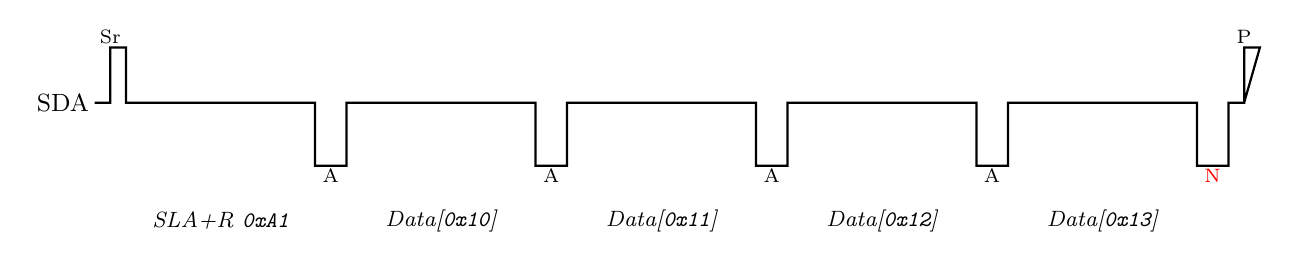
\begin{tikzpicture}[
    line/.style={thick},
    bit/.style={font=\scriptsize,inner sep=1pt},
    phase/.style={font=\footnotesize\itshape}
]

\draw[line]
    (0,1.5) -- (0.2,1.5) -- (0.2,2.2) node[bit,above]{Sr}
    -- (0.4,2.2) -- (0.4,1.5)
    -- (2.8,1.5) -- (2.8,0.7) -- (3.2,0.7) -- (3.2,1.5)
    -- (5.6,1.5) -- (5.6,0.7) -- (6.0,0.7) -- (6.0,1.5)
    -- (8.4,1.5) -- (8.4,0.7) -- (8.8,0.7) -- (8.8,1.5)
    -- (11.2,1.5) -- (11.2,0.7) -- (11.6,0.7) -- (11.6,1.5)
    -- (14.0,1.5) -- (14.0,0.7) -- (14.4,0.7) -- (14.4,1.5)
    -- (14.6,1.5) -- (14.6,2.2) node[bit,above]{P} -- (14.8,2.2) -- (14.6,1.5);

\node[phase] at (1.6,0.0) {SLA+R \hex{A1}};
\node[phase] at (4.4,0.0) {Data[\hex{10}]};
\node[phase] at (7.2,0.0) {Data[\hex{11}]};
\node[phase] at (10.0,0.0) {Data[\hex{12}]};
\node[phase] at (12.8,0.0) {Data[\hex{13}]};

\node[bit,below] at (3.0,0.7) {A};
\node[bit,below] at (5.8,0.7) {A};
\node[bit,below] at (8.6,0.7) {A};
\node[bit,below] at (11.4,0.7) {A};
\node[bit,below,red] at (14.2,0.7) {N};

\node[font=\small] at (-0.4,1.5) {SDA};
\end{tikzpicture}
\end{center}

每个字节后主控 ACK 表示还要继续，最后一个字节 NACK + STOP 结束。
地址溢出 \hex{3FFF} 后自动从 \hex{0000} 重新开始（wrap-around，与
24LC256 一致）。

\subsection{Clock Stretching：覆盖 Flash 写入}

主控在 STOP 后立即想做下一次读，但从机正在写 Flash（5--40 ms）。
\textbf{从机自动拉低 SCL}，主控的 START 信号被延迟到从机空闲：

\begin{center}
\begin{tikzpicture}[
    line/.style={thick}
]

\node at (-0.5,1.5) {SDA};
\draw[line] (0,1.5) -- (1.0,1.5) -- (1.0,2.3) node[font=\scriptsize,above]{STOP}
            -- (1.2,2.3) -- (1.2,1.5) -- (6.0,1.5)
            -- (6.0,2.3) node[font=\scriptsize,above]{START}
            -- (6.2,2.3) -- (6.2,1.5) -- (8,1.5);

\node at (-0.5,0.3) {SCL};
\draw[line] (0,0.7) -- (1.0,0.7);
\draw[line,red,decorate,decoration={zigzag,segment length=2mm,amplitude=0.2mm}]
            (1.0,0.7) -- (5.5,0.7);
\draw[line] (5.5,0.7) -- (5.5,1.2) -- (5.7,1.2) -- (5.7,0.7) -- (6.0,0.7);
\draw[line] (6.0,0.7) -- (6.0,1.2) -- (6.2,1.2) -- (6.2,0.7) -- (8,0.7);

\draw[<->,thick,blue!60!black]
    (1.0,-0.5) -- (5.5,-0.5)
    node[midway,below,blue!60!black,font=\footnotesize]
    {从机拉低 SCL，主控等待，约 5--40\,ms};

\node[font=\scriptsize,below=2.0cm,red] at (3.2,0.7) {Flash 擦写中};

\end{tikzpicture}
\end{center}

\textbf{从机怎么做到的}：TX32F01 的 I\textsuperscript{2}C 控制器在
\reg{CR.SI} 位置 1 时\textbf{自动拉低 SCL}，直到 ISR 把 SI 清掉。
我们 ISR 在 STOP 事件里如果发现有数据 pending，就先做 Flash 写入
再清 SI——主控全程透明等待。

\subsection{Page Write 边界回卷}

24LC128 的 Page = 64 字节。写超过页边界，地址自动回卷到本页起始：

\begin{center}
\begin{tikzpicture}[
    line/.style={thick},
    bit/.style={font=\scriptsize}
]

\draw[line] (0,2.0) -- (16,2.0);
\foreach \x/\addr in {0/0x0040, 2/0x0050, 4/0x0060, 6/0x0070, 8/0x0080, 10/0x0090, 12/0x00A0, 14/0x00B0, 16/0x00C0} {
    \draw[line] (\x,1.8) -- (\x,2.2);
    \node[font=\scriptsize,below] at (\x,1.8) {\addr};
}

\draw[line,red,thick] (0,2.5) -- (0,2.8) -- (8,2.8) -- (8,2.5)
    node[midway,above,font=\footnotesize,red]{Page 1 (\hex{0040}--\hex{007F})};

\draw[line,red,thick] (8,2.5) -- (8,2.8) -- (16,2.8) -- (16,2.5)
    node[midway,above,font=\footnotesize,red]{Page 2 (\hex{0080}--\hex{00BF})};

\draw[->,thick,blue!60!black] (5,1.4) -- (5,1.0)
    node[below,blue!60!black,font=\footnotesize]{主控写 70 字节从 \hex{0050}};

\draw[->,thick,green!50!black] (1.0,0.4) -- (1.5,0.4);
\node[font=\footnotesize,green!50!black,right] at (1.5,0.4)
    {前 48 字节正常写入 \hex{0050}--\hex{007F}};

\draw[->,thick,orange!80!black] (1.0,-0.1) -- (1.5,-0.1);
\node[font=\footnotesize,orange!80!black,right] at (1.5,-0.1)
    {第 49 字节起回卷到 \hex{0040}，覆盖之前的字节};

\end{tikzpicture}
\end{center}

我们严格遵守这个语义，主控驱动可以利用它实现"环形 page 内更新"等高级模式。

\section{协议状态机}

每个 I\textsuperscript{2}C 帧分两阶段。从机用 8 位状态码反映总线事件：

\begin{center}
\begin{tabular}{lll}
\toprule
\textbf{SR 值} & \textbf{含义} & \textbf{从机动作} \\
\midrule
\hex{60} & 收到 SLA+W，ACK & 重置 page buffer，准备接收 \\
\hex{80} & 收到数据字节，ACK & 累积到 page buffer（前 2 字节是地址） \\
\hex{88} & 收到数据字节，NACK & 同上，准备结束 \\
\hex{A8} & 收到 SLA+R，ACK & 从 addr\_ptr 取一字节 \\
\hex{B8} & 已发字节，主控 ACK & 继续从 addr\_ptr++ 取下一字节 \\
\hex{C0} & 已发字节，主控 NACK & 准备 STOP \\
\hex{C8} & 已发最后字节，主控 NACK & 同上 \\
\hex{D0} & 收到 STOP & 提交 page buffer 到 Flash（若有数据） \\
\bottomrule
\end{tabular}
\end{center}

状态机本身极简，所有"24Cxx 是这么工作的"业务规则集中在 \texttt{on\_stop()}
回调里——这正是 BSP / APP 分层的体现。

\subsection{状态流程图}

\begin{center}
\begin{tikzpicture}[
    state/.style={rectangle,draw,thick,rounded corners=2pt,minimum width=2.6cm,
                  minimum height=0.8cm,font=\small,fill=blue!8,align=center},
    arrow/.style={-{Stealth[length=2.5mm]},thick}
]

\node[state] (idle)       at (0,4) {IDLE};
\node[state] (got_w)      at (4,4) {WRITE 接收中};
\node[state] (got_addr)   at (8,4) {地址已获取};
\node[state] (got_r)      at (4,2) {READ 发送中};
\node[state] (stop)       at (4,0) {STOP（提交）};

\draw[arrow] (idle) -- node[above,font=\scriptsize]{SR=\hex{60}} (got_w);
\draw[arrow] (got_w) -- node[above,font=\scriptsize]{2 个字节后} (got_addr);
\draw[arrow] (got_addr.south) -- node[right,font=\scriptsize]{SR=\hex{D0}} (stop.north -| got_addr.south);
\draw[arrow] (idle) to[bend right=20] node[left,font=\scriptsize]{SR=\hex{A8}} (got_r);
\draw[arrow] (got_r) to[loop right] node[right,font=\scriptsize,align=left]{SR=\hex{B8}, 地址++} (got_r);
\draw[arrow] (got_r) -- node[right,font=\scriptsize]{SR=\hex{C0} / \hex{D0}} (stop);
\draw[arrow] (stop) -- node[left,font=\scriptsize]{Flash 写入完成} (idle);
\end{tikzpicture}
\end{center}

\section{加密区数据流}

\subsection{写入路径}

\begin{center}
\begin{tikzpicture}[
    node distance=0.6cm and 1.4cm,
    block/.style={rectangle,draw,thick,minimum width=2.6cm,minimum height=0.9cm,
                  font=\small,rounded corners=2pt},
    arrow/.style={-{Stealth[length=3mm]},thick}
]

\node[block,fill=blue!10]    (host) {Host I\textsuperscript{2}C write};
\node[block,fill=orange!10,right=of host] (emu)  {emu state machine};
\node[block,fill=purple!10,right=of emu]  (aes)  {AES-CTR XOR};
\node[block,fill=red!10,right=of aes]     (flash){Flash word program};

\draw[arrow] (host) -- node[above,font=\scriptsize]{\hex{0xDEADBEEF}} (emu);
\draw[arrow] (emu) -- node[above,font=\scriptsize]{addr in enc 区} (aes);
\draw[arrow] (aes) -- node[above,font=\scriptsize]{\hex{0xA347...}} (flash);

\node[font=\scriptsize,below=of aes,yshift=0.3cm] {Die ID 派生密钥};
\end{tikzpicture}
\end{center}

\subsection{读取路径}

\begin{center}
\begin{tikzpicture}[
    node distance=0.6cm and 1.4cm,
    block/.style={rectangle,draw,thick,minimum width=2.6cm,minimum height=0.9cm,
                  font=\small,rounded corners=2pt},
    arrow/.style={-{Stealth[length=3mm]},thick}
]

\node[block,fill=red!10]     (flash) {Flash byte};
\node[block,fill=purple!10,right=of flash] (aes)  {AES-CTR XOR};
\node[block,fill=orange!10,right=of aes]   (emu)  {emu state machine};
\node[block,fill=blue!10,right=of emu]     (host) {Host I\textsuperscript{2}C read};

\draw[arrow] (flash) -- node[above,font=\scriptsize]{\hex{0xA347...}} (aes);
\draw[arrow] (aes) -- node[above,font=\scriptsize]{\hex{0xDEADBEEF}} (emu);
\draw[arrow] (emu) -- node[above,font=\scriptsize]{透明明文} (host);
\end{tikzpicture}
\end{center}

主控读到的永远是明文。任何"芯片焊下来读 Flash"的人看到的永远是密文。

\subsection{攻击模型}

\begin{center}
\begin{tabular}{lll}
\toprule
\textbf{攻击方式} & \textbf{我们抗得住吗} & \textbf{为什么} \\
\midrule
拷贝 Flash dump 到另一片 chip & \textbf{抗} & Die ID 不同，密钥不同，解密失败 \\
反复读同一地址寻找规律     & \textbf{抗} & CTR nonce 每地址唯一 \\
监听 I\textsuperscript{2}C 总线        & \textcolor{red}{不抗} & 总线上是明文（本就是设计如此） \\
SCA / DPA 侧信道攻击      & \textcolor{red}{不抗} & 软件 AES 时间不恒定 \\
完整逆向固件 + Die ID 提取 & \textcolor{red}{不抗} & 拿到密钥派生算法 + Die ID 可复制 \\
\bottomrule
\end{tabular}
\end{center}

定位：\textbf{抗"无设备的攻击者"}，足以防止"把芯片焊下来拷贝 Flash 卖盗版"。
不能抗"完全控制设备 + 高级技术"的攻击。

\section{容量与性能}

\subsection{固件占用}

\begin{center}
\begin{tabular}{lr}
\toprule
\textbf{模块} & \textbf{ROM 估计} \\
\midrule
启动代码 + CRT  & 500\,B \\
AES-128 实现   & 1.5\,KB \\
存储抽象       & 0.7\,KB \\
I\textsuperscript{2}C 状态机 & 0.5\,KB \\
BSP（I\textsuperscript{2}C + UART） & 1.0\,KB \\
HAL 选用部分   & 1.5\,KB \\
main + 杂项    & 0.3\,KB \\
\midrule
\textbf{合计} & \textbf{\textasciitilde 6\,KB} \\
\bottomrule
\end{tabular}
\end{center}

预算 6 KB，留 2 KB 余量。

\subsection{时间预算}

\begin{center}
\begin{tabular}{ll}
\toprule
\textbf{操作} & \textbf{耗时} \\
\midrule
AES-128 块加密（单 block）            & \textasciitilde 145\,$\mu$s \\
1 字节读（明文区）                    & $<$ 1\,$\mu$s \\
1 字节读（加密区）                    & \textasciitilde 145\,$\mu$s \\
Flash 单 sector 擦除（512\,B）        & \textasciitilde 5\,ms \\
Flash 单 word 编程                    & \textasciitilde 30\,$\mu$s \\
完整 page write（64\,B，含擦写）      & \textasciitilde 8\,ms \\
\bottomrule
\end{tabular}
\end{center}

\section{测试方案}

\subsection{基本探测}

Linux 主机 + USB-I\textsuperscript{2}C 桥（CH341A / FT2232H / Bus Pirate）：

\begin{lstlisting}[language=bash]
sudo apt-get install i2c-tools
i2cdetect -y 1
# 应该在地址 0x50 看到设备
\end{lstlisting}

\subsection{读写回环}

\begin{lstlisting}[language=bash]
# 写 4 字节到地址 0x0010
i2cset -y 1 0x50 0x00 0x10 0x12 0x34 0x56 0x78 i

# 等 10 ms 让 Flash 完成写入
sleep 0.02

# 用随机读读回
i2cget -y 1 0x50 0x10 b
# 应该返回 0x12 (第一个字节)
\end{lstlisting}

\subsection{加密区验证}

\begin{enumerate}
    \item 主控写 \hex{0xCAFEBABE} 到地址 \hex{3F00}
    \item Keil debugger 暂停 CPU，读 Flash 物理地址 \hex{010057000}（=
          \hex{01001800} + \hex{3F00} - wait, 应该是 \hex{010047000} + \hex{3F00} = \hex{01004700}）
          实际：\hex{01001800} + \hex{3F00} = \hex{010057000}
    \item Flash 中应该是密文，\textbf{不是} \hex{0xCAFEBABE}
    \item 主控读 \hex{3F00} → 应该读回原始 \hex{0xCAFEBABE}
\end{enumerate}

\subsection{计数器验证}

\begin{lstlisting}[language=bash]
# 初始读取
i2cget -y 1 0x50 0x3F b ; i2cget -y 1 0x50 0xFC b
# 应该返回 0x00 0x00 (counter == 0)

# 触发 +1
i2cset -y 1 0x50 0x3F 0xFC 0x00 i

# 再读
i2cget -y 1 0x50 0x3F b ; i2cget -y 1 0x50 0xFC b
# counter == 1
\end{lstlisting}

\subsection{UART 实时统计}

UART 每秒一行输出：

\begin{lstlisting}
[I2CEE] up=12000ms  wr=24 rd=128 bytes=512 addr=0x3F00 counter=7
\end{lstlisting}

字段：芯片运行时间、累计写帧数、累计读帧数、累计字节数、最后访问地址、
当前计数值。

\section{已知限制}

\begin{itemize}
    \item \textbf{I\textsuperscript{2}C 最高时钟 400 kHz}：超过这个频率 ISR 跟不上字节速率。
          标准 24LC256 fast-mode 也是这个值，所以兼容主流主控。
    \item \textbf{每次 STOP 都触发 Flash 擦写}：写入吞吐受 Flash 擦写时间限制。
          多次小写比一次大写慢得多。这是真实 EEPROM 也有的限制。
    \item \textbf{无写保护}：BP 位、WC 引脚等都没实现。后续可以加。
    \item \textbf{加密强度有限}：密钥派生算法不是 KDF 强度，靠的是"Die ID 保密"。
\end{itemize}

\section{后续扩展}

每个都是 200--400 行的独立工作：

\begin{enumerate}
    \item \textbf{多 bank}：响应多个 I\textsuperscript{2}C 地址，每地址独立存储区。
    \item \textbf{写保护硬件引脚}（WP）：GPIO 输入低 = 禁止写入。
    \item \textbf{访问日志}：每次访问记录到隐藏区，主控不可见，供取证。
    \item \textbf{ECDH 协商会话密钥}：主控和从机用 ECDH 握手，会话内使用一次性密钥。
    \item \textbf{Flash wear leveling}：扩到外部 SPI NOR backing，10 万擦写寿命变 1000 万。
\end{enumerate}

\section{文件清单}

\begin{center}
\begin{longtable}{ll}
\toprule
\textbf{文件} & \textbf{作用} \\
\midrule
\endhead
\texttt{USER/main.c}                & 入口、初始化、1 秒心跳日志 \\
\texttt{EEPROM/eeprom\_protocol.h}  & 24Cxx 协议常量、区域定义 \\
\texttt{EEPROM/eeprom\_emu.h/.c}    & 协议状态机 \\
\texttt{EEPROM/eeprom\_storage.h/.c} & 存储抽象（加密 + counter） \\
\texttt{EEPROM/eeprom\_crypto.h/.c} & AES-128 + CTR 软件实现 \\
\texttt{BSP/bsp\_i2c\_slave.h/.c}   & I\textsuperscript{2}C 从机硬件 + ISR \\
\texttt{BSP/bsp\_uart.h/.c}         & 调试 UART \\
\texttt{TX32F01\_I2CEEPROM.sct}     & 链接脚本 \\
\texttt{TX32F01\_I2CEEPROM.uvprojx} & Keil 工程 \\
\texttt{doc/app\_i2ceeprom\_design.tex} & 本文档 \\
\bottomrule
\end{longtable}
\end{center}

\end{document}
